\documentclass[convert]{standalone}

\usepackage{tikz}

\tikzstyle{lines}=[%
	every path/.style = {
		fill = white,
		line width = 1.5pt
	}
]


\begin{document}
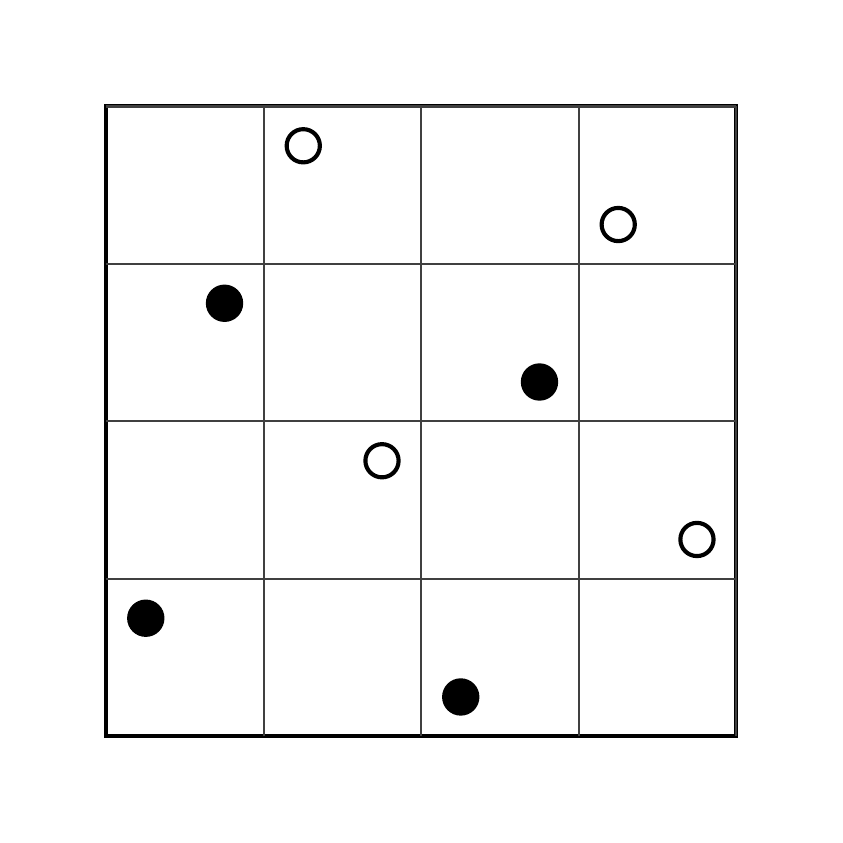
\begin{tikzpicture}[lines]
	\def\size{8}
	
	% Background, frame
	\draw[draw=none] (-0.5,-0.5) rectangle ++({\size+2},{\size+2});
	\draw (0.5,0.5) rectangle ++(\size,\size);

	% % Lines
	\begin{scope}[shift={(0.5,0.5)}]
		\foreach \y in {2,4,6,8} {
			\draw[darkgray, thick] (0, \y) -- ++(\size, 0);
			\draw[darkgray, thick] (\y, 0) -- ++(0, \size);
		}
	\end{scope}

	% % Points
	\foreach \x/\y in {1/2, 2/6, 5/1, 6/5} {
		\draw [fill=black] (\x,\y) circle (6pt);
	}
	\foreach \x/\y in {3/8, 4/4, 7/7, 8/3} {
		\draw (\x,\y) circle (6pt);
	}
	
\end{tikzpicture}
\end{document}